\chapter{Quantum Device Fabrication}\label{cha:appendix1}


During my Master's studies, I was trained by Timothy Child on the necessary fabrication steps to add inner and outer gates forming the quantum devices. Once fully qualified, I fabricated some devices on my own. There are a number of required steps to turn the GaAs/AlGaAs heterostructures received from Michael Manfra's group into a chip that we can then add the inner and outer gates. It should also be noted that I made no contribution to the nano fabrication recipes and simply followed the procedure developed by previous students. The following summary is largely adapted from Owen Sheekey's thesis, a past student from the Quantum Devices Group. 

\section{Summary}
The GaAs substrates are grown by Michael Manfra’s group at Purdue University. There are two key features to devices built on GaAs/AlGaAs 2DEGs – ohmic contact to the 2DEG and gating structures. In overview, devices used for this project use a thin film of $\mathrm{Al_2O_3}$ to electrically isolate top gates fabricated from Au/Ti. Ohmic contacts are made using annealed Ni/Au/Ge.

The general process of preparation of a sample goes as follows:

\begin{enumerate}
\item Gallium removal from back of wafers.
\item Ohmic contact: Lithography, evaporation, annealing.
\item Mesa etching: Lithography, $\mathrm{H_2SO_4}$ etching.
\item Atomic layer deposition: $\mathrm{Al_2O_3}$.
\item Gating (2 steps): Lithography, evaporation.
\item Wire bonding
\end{enumerate}

\section{Recipes}

\subsection{Gallium Removal}
This is a recipe developed by Dr. Silvia Lüscher Folk.


\begin{enumerate}
\item Cleave a full wafer into a quarter or half wafer. Blow off any dust bunnies from the surface before starting.
\item Spin a layer of AZ1518 resists at $4000 \,\mathrm{RPM}$ for $40\,\mathrm{s}$.
\item Bake the resist for $2\,\mathrm{minutes}$ at $100^\circ$C.
\item Put a clean wipe on a hotplate and set to $50^\circ$C. Put wafer face down (gallium side up) onto the clean wipe.
\item Wipe off gallium with q tips. Keep wiping until it is all gone.
\item Spin and bake another layer of AZ1518 ($4000 \,\mathrm{RPM}$ $40\,\mathrm{s}$ and bake $100^\circ$C $2\,\mathrm{minutes}$).
\item Etch $2 \,\mathrm{minutes}$ in full strength HCl. Quench etch by transferring to DI water.
\item Rinse well in DI water. Blow dry.
\item Squirt down with Acetone to strip resist from the surface and immediately rinse with IPA.
\item Soak 3~minutes each in Toluene, Acetone, and IPA. Rinse with IPA and blow dry between each solvent. Spray down with DI water and blow dry.
\end{enumerate}

\subsection{Mesa Etch}
\begin{enumerate}
\item Solvent clean – Acetone, IPA. Rinse in DI, blow dry with $\mathrm{N_2}$.
\item Prebake chip for \qty{60}{s} at $110^\circ$C.
\item AZ5214-E in positive mode, ramp up 500 RPM for \qty{2}{s}, spin at 4444 RPM for \qty{40}{s} with \qty{60}{s} softbake at $100^\circ$C.
\item Photo lithography in MLA150 Heidelberg (Maskless Aligner) : Expose \qty{90}{mJ/cm^2}, defocus -1 
\item Develop in MIF 300, $50\,\mathrm{s}$ stop develop in DI.
\item Hardbake for \qty{60}{s} at $120^\circ$C.
\item O2 plasma etch in Plasma etch PE 50, 60s.
\item Etch in $30\,\mathrm{mL}$ diluted Sulfuric acid (700 Water:3 $\mathrm{H_2S0_4}$) + $2 \,\mathrm{mL}$ $\mathrm{H_2O_2}$ at $18^\circ$C for \qty{50}{s}
\item Stop etch in DI water. Remaining resist can be removed with Acetone, IPA and DI.
\end{enumerate}




\subsection{Ohmic Contact}

\subsubsection{Lithography and Evaporation}


At the end of my Master's studies, there was a sizeable effort (that I was not involved in) to develop low resistance ohmic contacts by Vahid Mohaved and Dr. Silvia Lüscher Folk. Here is the most up to date recipe. 


\begin{enumerate}
\item Solvent clean – Acetone, IPA, Ultrasound. Rinse in DI, blow dry with $\mathrm{N_2}$.
\item Dehydration bake chip for $1 \,\mathrm{minutes}$ at $110^\circ$C.
\item AZ5214-E in image reversal mode, ramp up 500 RPM for \qty{2}{s}, spin at 4444 RPM for \qty{50}{s} with \qty{60}{s} softbake at $90^\circ$C.
\item Photo lithography in MLA150 Heidelberg (Maskless Aligner) : Expose \qty{40}{mJ/cm^2}, defocus +1 
\item IR bake for \qty{30}{s} at $110^\circ$C.
\item Photo lithography in MLA150 Heidelberg : Flood exposure \qty{222}{mJ/cm^2}, defocus +1 
\item Develop in AZ300 MIF , $40\,\mathrm{s}$ stop develop in DI.
\item Hardbake for \qty{60}{s} at $110^\circ$C.
\item $\mathrm{O^2}$ plasma etch in Plasma etch PE 50, $15\,\mathrm{s}$.
\item Dip in $37\%$ HCI for \qty{20}{s}. Rinse with DI for \qty{120}{s}

\item Evaporate the following:

\begin{table}[H] 
\centering
 \begin{tabular}{|p{2.0cm}|p{2.0cm}|p{2.0cm}|}
 \hline
 Metal & Thickness & Rate\\
 \hline
 Ni & $7\,\mathrm{nm}$ & $1.0\,\mathrm{\dot{A}s^{-1}}$\\
 Ge & $80\,\mathrm{nm}$ & $1.3\,\mathrm{\dot{A}s^{-1}}$\\
 Au & $160\,\mathrm{nm}$ & $2.0\,\mathrm{\dot{A}s^{-1}}$\\
 Ni & $36\,\mathrm{nm}$ & $1.6\,\mathrm{\dot{A}s^{-1}}$\\
 Au & $80\,\mathrm{nm}$ & $1.7\,\mathrm{\dot{A}s^{-1}}$\\
 \hline
 \end{tabular}
\label{tab:ohmic_evaporation}
\end{table}
\item Liftoff in Acetone at $70^\circ$C.
\item Rinse in Acetone, IPA and blowdry with $\mathrm{N_2}$.
\end{enumerate}



\subsubsection{Annealing}
The following process was followed on the rapid thermal annealer made “in house” for annealing GaAs and other substrates. The basic idea is to use a bulb in a near vacuum (with some amount of forming gas – $\mathrm{H_2}$ + $\mathrm{N_2}$) to heat the sample to a high temperature for a limited amount of time. The metal film melts and diffuses through the GaAs substrate to make contact with the 2DEG, usually $30-200\,\mathrm{nm}$ below the surface.

\begin{enumerate}
\item Pump down should reach lower limit, $0.133\,\mathrm{mbar}$.
\item Set regulator to $2.5\,\mathrm{psi}$ (forming gas).
\item Open Swagelock valve until pressure reads $10\,\mathrm{mbar}$.
\item Close speedivalve until pressure reads $200\,\mathrm{mbar}$.
\item Turn on bulb to roughly $34\,\%$, it takes about $5-10\,\mathrm{minutes}$
\item Wait at $350^\circ$C for $2\,\mathrm{minutes}$
\item Go to $450^\circ$C as fast as you can, hold it there for $40\,\mathrm{s}$.
\item Cool below $300^\circ$C fast by opening the speedivalve on the pump line all the way, and opening the gas flow.
\item Cool to $50^\circ$C, then vent and let cool to room temperature.
\end{enumerate}


\subsection{Gating}
% \label{appendix:fab_gates}

Gating is the process of adding metal to the top of the GaAs/AlGaAs heterostructure, which are then used to form and control the potential landscape in the 2DEG below (Fig.~\ref{fig:appx/gate_fab}). The overall recipe for gating was not varied during my fabrication time. However, if long periods have passed between fabrication (a few months), it is necessary to test an array of exposure doses for the E beam step as this parameter can vary over long periods of time and system re starts.





\subsubsection{Inner Gates}

\begin{enumerate}
\item Solvent clean - Acetone, IPA. Rinse in DI, blow dry with $\mathrm{N_2}$.
\item Prebake chip for $3\,\mathrm{minutes}$ at $180^\circ$C.
\item Spin PMMA A2 495K at $5555\,\mathrm{RPM}$ for $50\,\mathrm{s}$ with $3\,\mathrm{minutes}$ bake at $180^\circ$C
\item Spin PMMA A1 950K at $3333\,\mathrm{RPM}$ for $50\,\mathrm{s}$ with $5\,\mathrm{minutes}$ bake at $180^\circ$C
\item E beam lithography in Jeol JBX 8100FS : Dose \qty{900}{\micro C/cm^2}
\item Develop in IPA:DI, 7:3 $40\,\mathrm{s}$ at $18^\circ$C, stop by directly drying with $\,\mathrm{N_2}$.
\item Evaporate Ti $3\,\mathrm{nm}$, $1.5\,\mathrm{\dot{A}s^{-1}}$ then Au $12\,\mathrm{nm}$ $4\,\mathrm{\dot{A}s^{-1}}$.
\item Liftoff in Acetone at room temperature.
\end{enumerate}



\begin{figure}[!bht]
 \begin{center}
%% includegraphics: comment the following if not using the graphicx package
 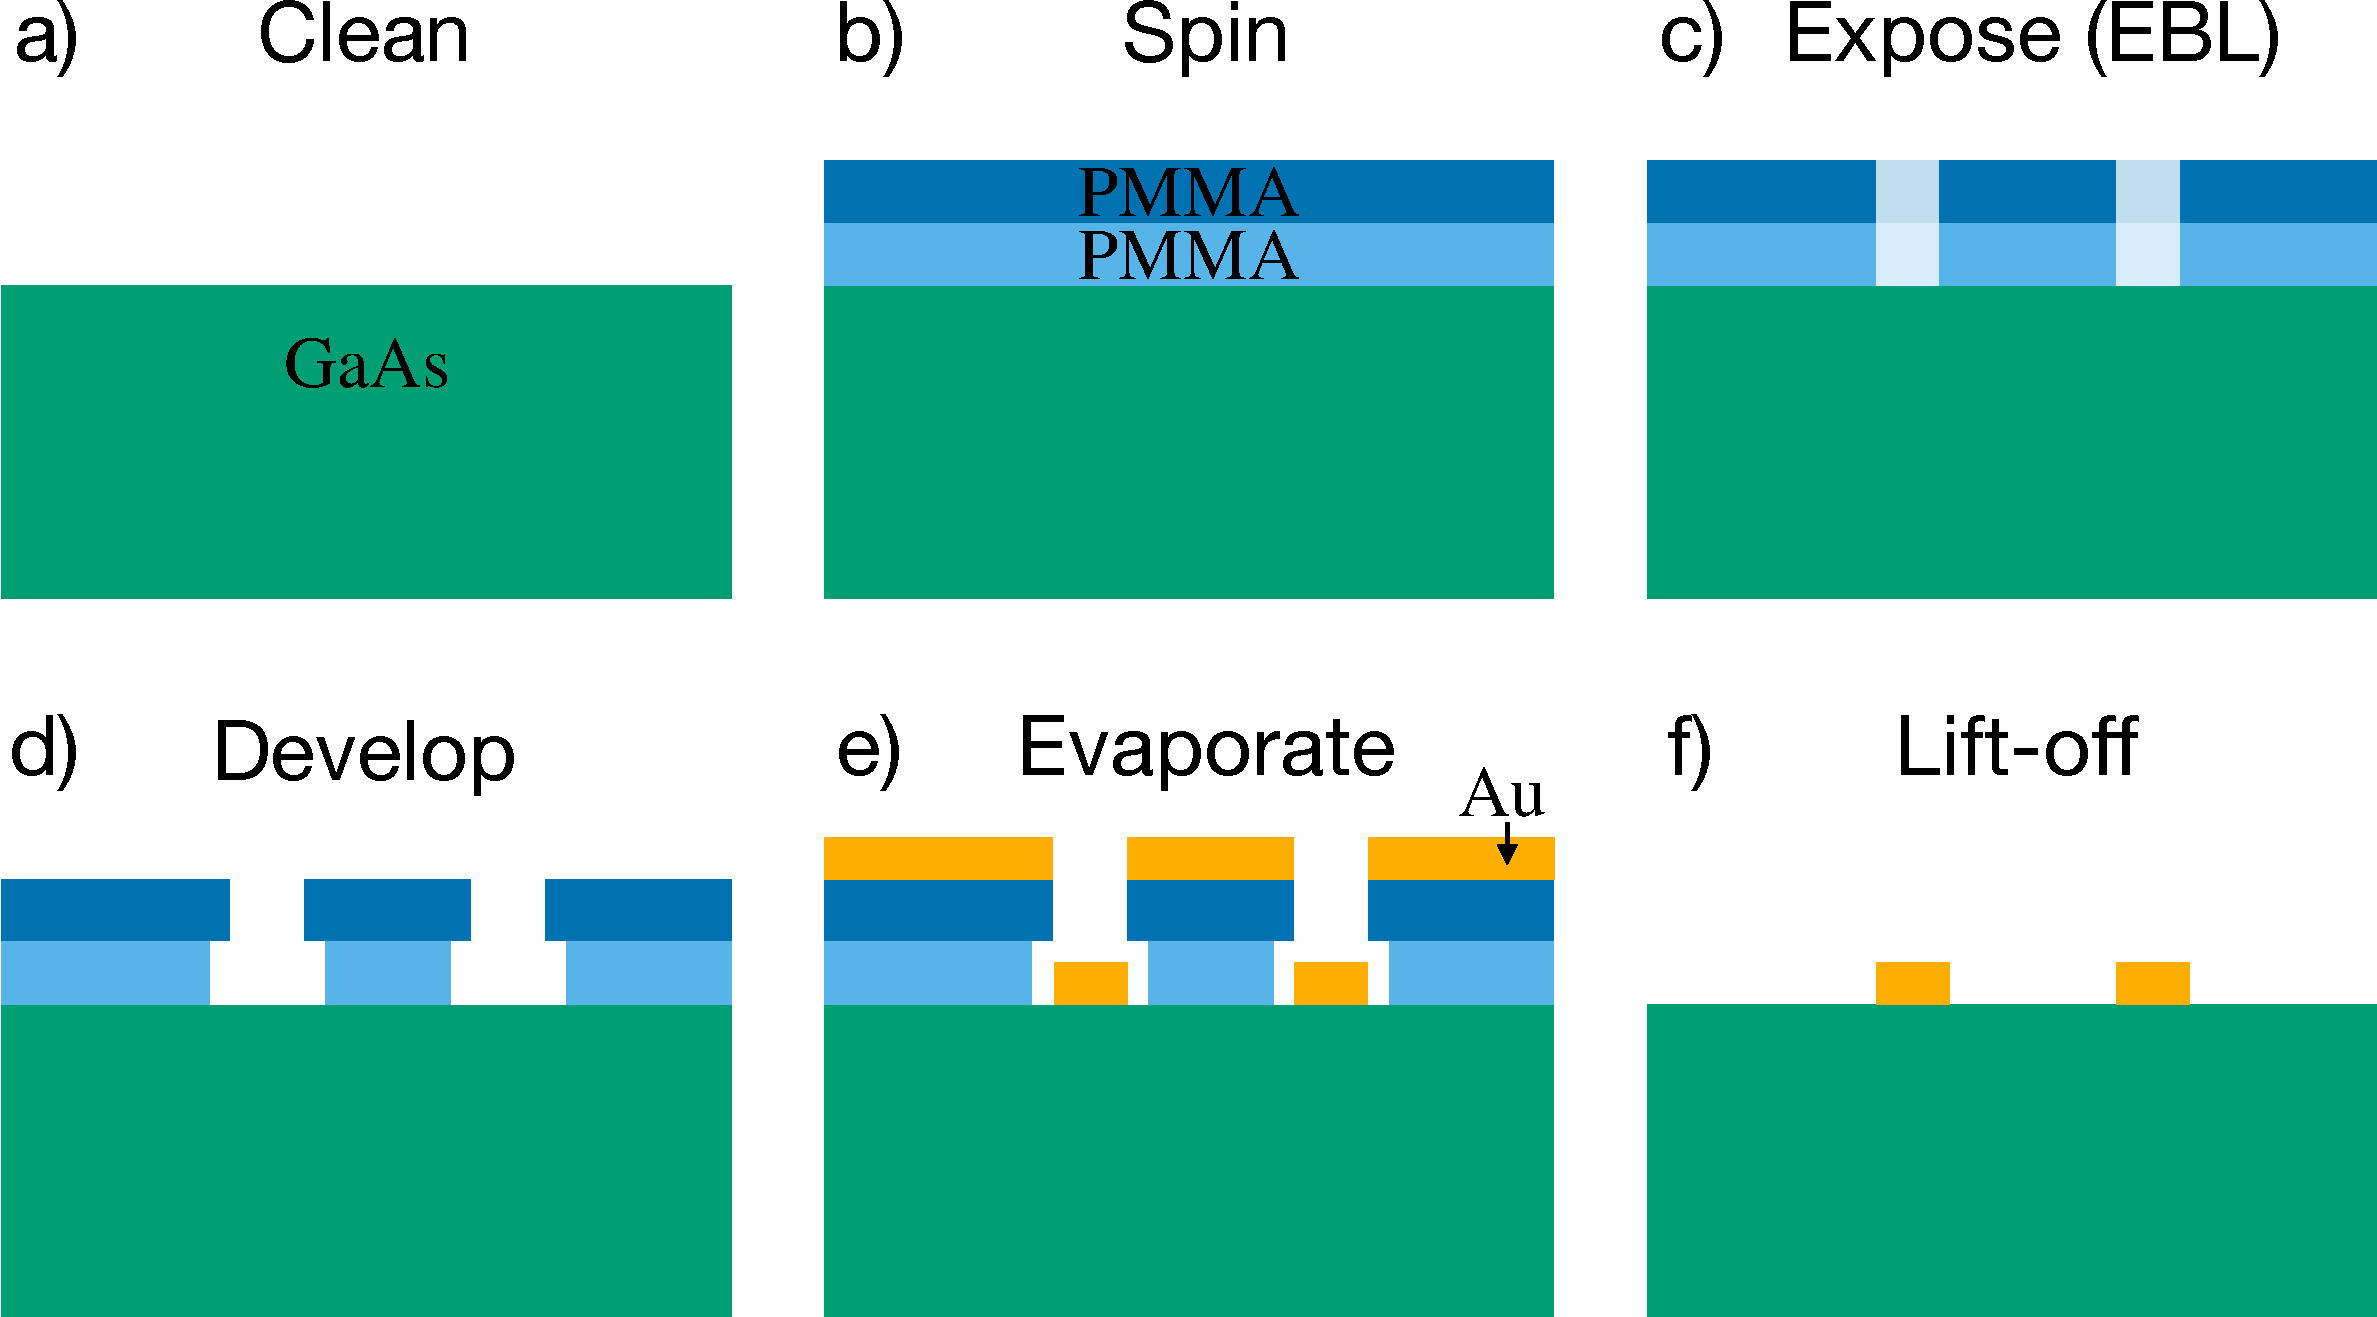
\includegraphics[width=1.0\textwidth]{figures/appendix/figure20.pdf}
 \caption[Gate Fabrication Illustration]{\label{fig:appx/gate_fab} 
 (\textbf{a}) GaAs/AlGaAs heterostructure is cleaned in an Ultra Sonic (US) bath with acetone/IPA/DI. 
 (\textbf{b}) Two different layers of PMMA are spun ontop of the heterostructure.
 (\textbf{c}) The gate design is exposed to an electron beam to breakup the PMMA.
 (\textbf{d}) The chip is developed in an IPA:DI solution create an undercut and remove the exposed PMMA.
 (\textbf{e}) 2:\qty{12}{nm} of Ti:Au are evaporated ontop of the chip.
 (\textbf{f}) The chip is rinsed in acetone to remove remaining PMMA and any metal attached to it. The chip is ready to be placed onto a chip carrier, wirebonded and measured.}
 \end{center}
\end{figure}



\subsubsection{Outer Gates and Bondpads}

\begin{enumerate}
\item Solvent clean – Acetone, IPA. Rinse in DI, blow dry with $\mathrm{N_22}$.
\item Prebake chip for $3\,\mathrm{minutes}$ at $180^\circ$C.
\item Spin PMMA A8 495K at $4000\,\mathrm{RPM}$ for $40\,\mathrm{s}$ with $3\,\mathrm{minutes}$ bake at $180^\circ$C
\item Spin PMMA A4 490K at $4000\,\mathrm{RPM}$ for $40\,\mathrm{s}$ with $5\,\mathrm{minutes}$ bake at $180^\circ$C
\item E beam lithography in Jeol JBX 8100FS : Dose \qty{1100}{\micro C/cm^2}
\item Develop in IPA:DI, 7:3 $40\,\mathrm{s}$ at $18^\circ$C, stop in DI.
\item $\mathrm{O_2}$ plasma etch in Plasma etch PE 50, $1\,\mathrm{minutes}$.
\item Evaporate Ti $10\,\mathrm{nm}$, $2\,\mathrm{\dot{A}s^{-1}}$ then Au $100\,\mathrm{nm}$, $4\,\mathrm{\dot{A}s^{-1}}$.
\item Liftoff in Acetone at room temperature.
\end{enumerate}




\subsection{Wire Bonding}

The final step in the fabrication process is to attach the chip to a chip carrier and connect the gates and ohmic contacts to bond pads (Fig.~\ref{fig:appx/wirebond}). The chip carrier is added to the fridge and connected to the fridge wiring, which leads to a break-out box outside the fridge. 


\begin{enumerate}
\item Stick the chip to the chip carrier using a small dab of PMMA A8 495K. Bake for $5\,\mathrm{minutes}$ at $60^\circ$C
\item Wirebond bond pads on chip carrier to gates and ohmic contacts on the chip:
\begin{table}[H] 
\centering
 \begin{tabular}{|p{3.0cm}|p{2.0cm}|p{2.0cm}|}
 \hline
 & Bond 1 & Bond 2\\
 \hline
 Wire material & Al & Al\\
 Bond strength & 260 & 300\\
 Bond duration & \qty{30}{ms} & \qty{30}{ms} \\
 \hline
 \end{tabular}
\label{tab:wire_bonding}
\end{table}
\end{enumerate}


\begin{figure}[!bht]
 \begin{center}
%% includegraphics: comment the following if not using the graphicx package
 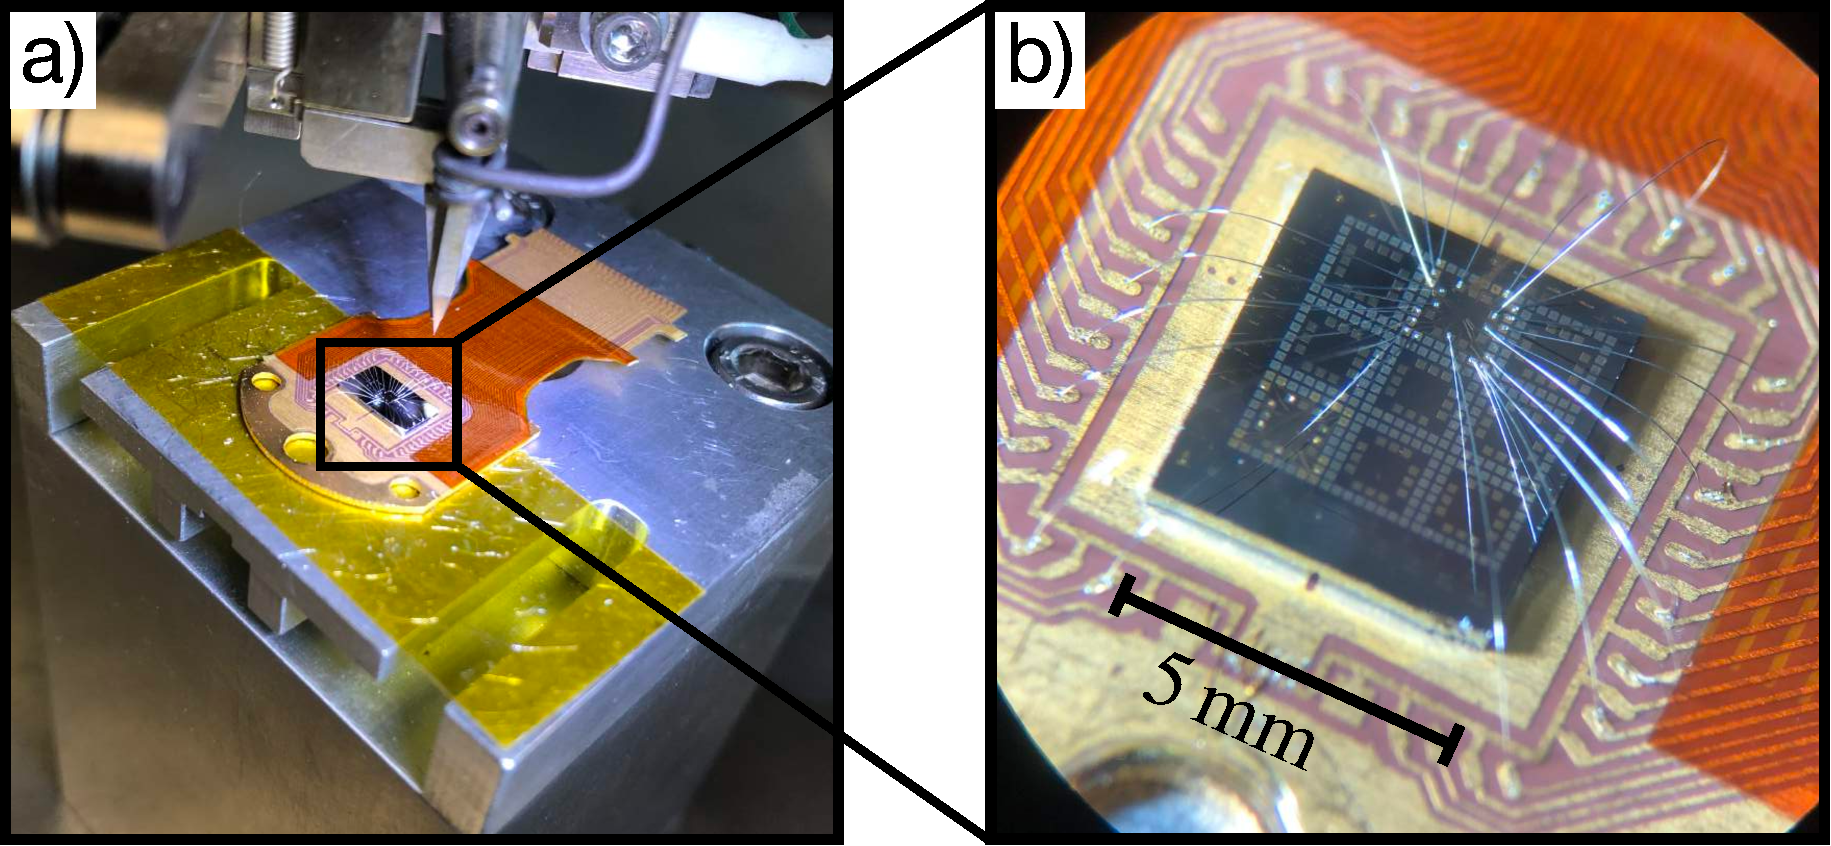
\includegraphics[width=1.0\textwidth]{figures/appendix/figure21.pdf}
 \caption[Wirebonding a Chip]{\label{fig:appx/wirebond} 
 (\textbf{a}) Chip carrier stuck to a platform under the wirebonder. (\textbf{b}) Close-up of the Al wire bonds that connect the device gates to a chip carrier.}
 \end{center}
\end{figure}